\chapter{Allgemeines}
\section{�berblick}

Das Campus Informationssystem ist die zentrale Web-Oberfl�che f�r Studierende und MitarbeiterInnen. Hier werden verschiedene Servicedienste zur Verf�gung gestellt.
Hier finden Sie News, k�nnen sich �ber die Lehre informieren, Lehrveranstaltungspl�ne abrufen und vieles mehr. 

\begin{figure}
	\centering
	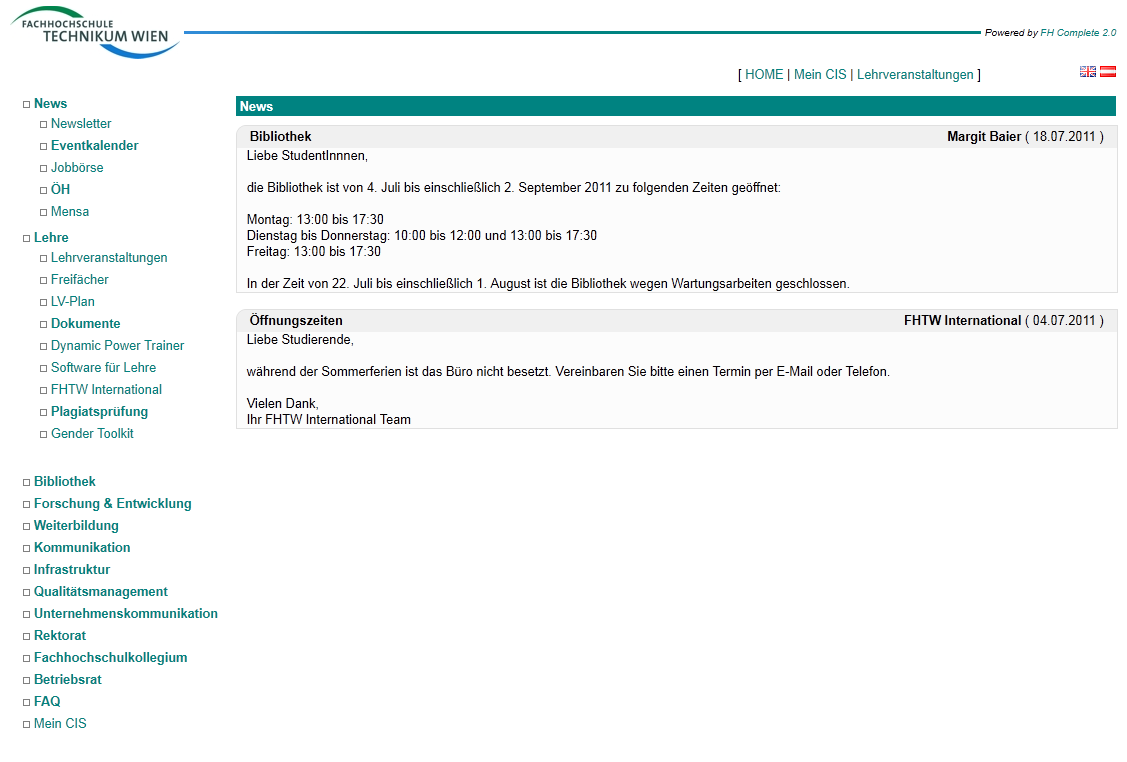
\includegraphics[width=0.70\textwidth]{CIS_Startseite.png}
	\caption{CIS Startseite}
	\label{CIS_startseite}
\end{figure}

\section{Hauptmen�punkte}

	\minisec{News}
Im CIS gibt es verschieden Ansichten f�r News (im Bereich der LV-News auch Pinboard genannt). Auf der Startseite befindet sich die Ansicht f�r "`allgemeine News"'. Des weiteren gibt es Ansichten f�r die einzelnen Organisationseinheiten (Studiengang, Institut, ...). Diese werden auf den entsprechenden Unterseiten angezeigt und dort mit den allgemeinen News gemischt.
Die Richtlinien zur Newsverwaltung entnehmen Sie bitte  Kapitel \ref{richtlinien_newseintraege}

Der Abschnitt "`News"' im CIS beinhaltet auch Links zu anderen externen News und Informationsplattformen.

	\minisec{Lehre}
Der Bereich Lehre umfasst alle notwendigen Informationen und Unterlagen zur Durchf�hrung der Lehre wie Infos zu Lehrveranstaltungen, Anwesenheitslisten, Notenlisten, TeilnehmerInnenlisten, Mailgruppen, Semesterplan und das Abgabetool zur leichteren Durchf�hrung von �bungen.

Au�erdem kann man sich in diesem Bereich f�r Freif�cher anmelden und findet Tools und Informationen zur Durchf�hrung der Lehre.
Details dazu entnehmen Sie bitte dem Kapitel \ref{lehre}.

	\minisec{Bibliothek}
Hier finden Sie Informationen zur Bibliothek, Recherche-Links, Verweise zu elektronischen Medien und externen Literaturdatenbanken sowie die Publikationsdatenbank OPUS.

	\minisec{Forschung \& Entwicklung}
Informationen zu laufenden Projekten sowie Dokumente und Prozessabl�ufe f�r die Durchf�hrung von Forschungsprojekten sind unter diesem Men�punkt zu finden.

	\minisec{Weiterbildung}
Hier k�nnen Sie sich �ber das aktuelle interne und externe Weiterbildungsprogramm informieren.

	\minisec{Kommunikation}
Hier k�nnen Kontakte, eine Personensuche, das Webmail und Mailverteiler der FHTW abgerufen werden.

	\minisec{Infrastruktur}
Im Bereich Infrastruktur sind die wichtigsten Informationen rund um die technische und logistische Infrastruktur im Haus gesammelt:
Anleitungen und Tools zur Registration im LAN und WLAN, ein kostenloses Anti-Viren Programm, Infos zur Medienausstattung, Lagepl�ne sowie Verordnungen.

	\minisec{Qualit�tsmanagement}
Hier finden Sie alle studienrelevanten Dokumente und Prozessabl�ufe und Dokumente zur allgemeinen Organisation der FHTW sowie die relevanten Dokumentvorlagen.

	\minisec{Unternehmenskommunikation}
In diesem Men�punkt stehen das Logo der FHTW, Corporate Identity Handb�cher und ein Veranstaltungsleitfaden zum Download zur Verf�gung.

	\minisec{Rektorat}
Unter "`Rektorat"' finden Sie das Leitbild der FHTW, Kennzahlen, Gender Mainstreaming-Aktivit�ten, Hochschulprojekte, Auszeichnungen sowie Infos zu Wettbewerbsausschreibungen und Stipendien.

	\minisec{Fachhochschulkollegium}
	In diesem Men�punkt sind die Zusammensetzung und Gesch�ftsordnung des Kollegiums der FH Technikum Wien sowie relevante Dokumente dargestellt.

	\minisec{Betriebsrat}
News, Informationen und wichtige Dokumente wie z.B. Betriebsvereinbarungen sind hier zu finden.

	\minisec{FAQ}
Der Bereich FAQ (Frequently Asked Questions) bietet diverse Anleitungen, L�sungen zu h�ufig auftretenden Problemen, Handb�cher sowie den Link zum Archiv.

	\minisec{Mein CIS}
Unter diesem Abschnitt finden Sie gesammelt alle Informationen zu Ihrer Person und auch administrative Tools:
ein �berblick �ber Ihre Profildaten, Ihr pers�nlicher LV-Plan, Zeitw�nsche, das Urlaubstool (f�r MitarbeiterInnen), Ihre Lehrveranstaltungen (f�r LektorInnen) und Tools zur Bachelor- und Diplomabgabe.